\documentclass{iopjournal}

\usepackage{amsmath}
\usepackage{amssymb}
\usepackage{graphicx}
\usepackage{hyperref}

\begin{document}

\articletype{Letter}

\title{Statistical Mechanics of the $N$-Queens Lattice Gas: Monte Carlo Determination of the Simkin Constant}

\author{Zong-Yue Liu$^{1}$ and Lei Wang$^{2,*}$}

\affil{$^1$Department of Physics, Nanjing University, Nanjing 210093, China}

\affil{$^2$Institute of Physics, Chinese Academy of Sciences, Beijing 100190, China}

\affil{$^*$Author to whom any correspondence should be addressed.}

\email{wanglei@iphy.ac.cn}

\keywords{$N$-queens problem, lattice gas, Monte Carlo simulation, combinatorial entropy}

\begin{abstract}
We investigate the $N$-queens problem as a lattice gas in which
$N$ queens are placed on an $N \times N$ chessboard with pairwise
repulsive interactions along shared rows, columns, and diagonals.
The ground states are exactly the $Q(N)$ solutions of the classical
$N$-queens problem, whose entropy per queen
$s_0 \approx \ln N - \gamma$ ($\gamma \in [1.939,\, 1.945]$)
exhibits a characteristic constraint hierarchy: each successive
geometric constraint reduces the entropy from the free-placement
value $\ln N$ by a definite constant.
We derive the exact high-temperature energy $E/N \to 5/3$ as
$N \to \infty$.
Extensive Monte Carlo simulations for $N = 8$--$512$ reveal that
the specific heat per queen $C_v/N$ converges to a universal
function of temperature with a non-divergent peak
$C_v^{\max}/N \approx 1.62$ at $T^* \approx 0.237\,J$,
establishing the absence of a thermodynamic phase transition.
Thermodynamic integration of $C_v/T$ from $T = \infty$ to $T = 0$
recovers the ground-state entropy and yields the Simkin constant
$\gamma_{\rm MC} = 1.94$ at $N = 512$, within $0.1\%$ of the
combinatorial value, providing the first physical determination of
this fundamental constant.
\end{abstract}

\maketitle


%=====================================================================
The $N$-queens problem---placing $N$ mutually non-attacking queens
on an $N \times N$ chessboard---is among the oldest combinatorial
problems, dating back to Bezzel in 1848~[1].  Despite its long
history, the asymptotic enumeration of solutions was resolved only
recently.  Simkin~[2] proved that the number of solutions $Q(N)$
satisfies
\begin{equation}
  Q(N) \sim \left(\frac{N}{e^{\gamma}} \right)^N, \quad
  \gamma \in [1.939,\, 1.945],
  \label{eq:QN}
\end{equation}
building on the breakthroughs of Bowtell and Keevash~[3] and
Luria and Simkin~[4].  Simkin's proof introduces
\emph{queenons}---limit objects defined as probability measures on
the unit square---and characterizes $\gamma$ as the solution of a
convex optimization problem; the determination is purely
combinatorial.  Equation~(\ref{eq:QN}) yields a ground-state
entropy per queen
$s_0 = \lim_{N \to \infty} \ln Q(N)/N = \ln N - \gamma$.

The form of $s_0$ is physically suggestive.  On an $N \times N$
lattice, a single particle placed freely in one row has $\ln N$
units of entropy.  The $N$-queens entropy
$s_0 = \ln N - \gamma$ can be read as: each queen retains the full
lattice entropy, reduced by a constant $\gamma$ encoding the
cumulative cost of geometric constraints.  This constant decomposes
through a hierarchy of increasing stringency~[5]:
(i)~free placement (row constraint only) gives
$\Omega = N^N$, $s = \ln N$;
(ii)~permutation (row~+~column) gives
$\Omega = N!$, $s \approx \ln N - 1$;
(iii)~the $N$-queens constraint (row~+~column~+~two diagonals)
gives $\Omega \approx (N/e^\gamma)^N$,
$s \approx \ln N - \gamma$.
The column constraint costs exactly one unit of entropy (the
Stirling correction); the two diagonal constraints together cost
$\gamma - 1 \approx 0.94$ units.  That each geometric constraint
reduces the per-queen entropy by a constant independent of $N$
hints at a deeper statistical-mechanical structure underlying the
combinatorics.

This observation motivates the present work.  We embed the
$N$-queens problem in a lattice gas with tunable temperature and
perform extensive Monte Carlo (MC) simulations.  A central finding
is that thermodynamic integration of the specific heat recovers the
ground-state entropy---and hence $\gamma$---purely from MC data,
providing the first \emph{physical} route to this combinatorial
constant.

\textit{Model.}---We consider an $N \times N$ square lattice with
open boundary conditions.  Each site $(i,j)$ carries an occupation
variable $n_{ij} \in \{0,1\}$.  The Hamiltonian counts mutually
attacking queen pairs:
\begin{equation}
  H = \sum_{\alpha \in \mathcal{L}} \binom{n_\alpha}{2},
  \label{eq:H}
\end{equation}
where $\mathcal{L}$ denotes the set of all $6N - 2$ attack lines
($N$ rows, $N$ columns, $2N{-}1$ main diagonals, $2N{-}1$
anti-diagonals), $n_\alpha$ is the number of queens on line
$\alpha$, and $\binom{n}{2} = n(n{-}1)/2$.  We set $J = 1$ and
$k_B = 1$ throughout.  We work in the canonical ensemble with
fixed particle number $N$ and use Kawasaki dynamics~[6]
(queen--vacancy exchange) with the Metropolis acceptance
criterion~[7].  One sweep consists of $N$ attempted exchanges.
We simulate $N = 8$, 16, 32, 64, 100, 128 with $10^8$ measurement
sweeps per temperature point (318 temperatures spanning
$T = 0.05$--$400\,J$), preceded by $2 \times 10^6$ thermalization
sweeps.  Additional simulations at $N = 256$ and 512 use a
126-point temperature grid optimized for the entropy integration.
The schematic of the model is shown in Fig.~\ref{fig:schematic}.

\begin{figure}[t]
  \centering
  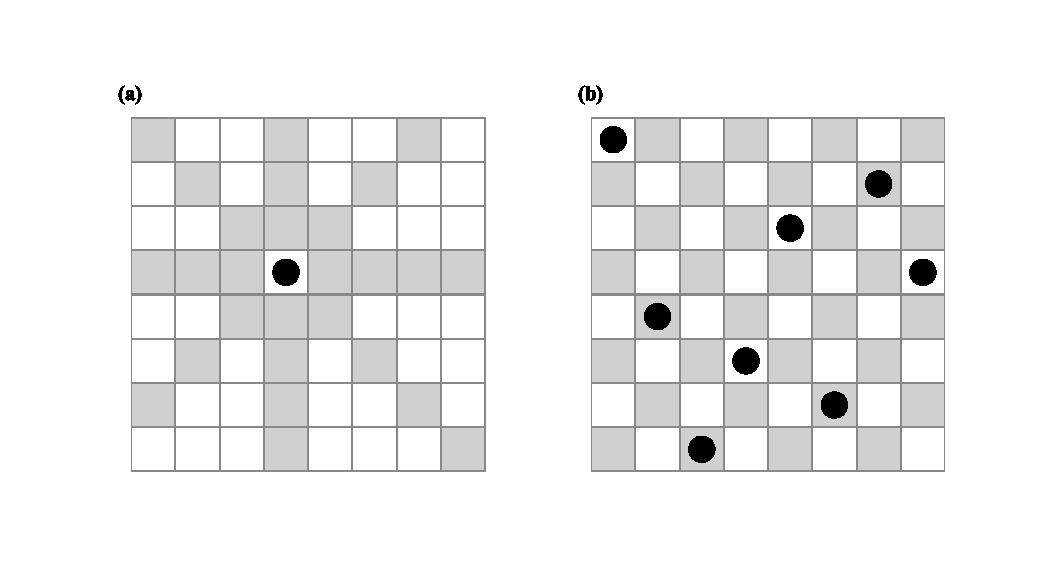
\includegraphics[width=0.9\linewidth]{fig1_schematic.pdf}
  \caption{(a)~A single queen (black circle) on an $8 \times 8$
  board; gray squares are attacked along the row, column, and two
  diagonal directions.
  (b)~One of the $Q(8) = 92$ non-attacking ground-state
  configurations.}
  \label{fig:schematic}
\end{figure}

\textit{Exact high-temperature limit.}---At $T \to \infty$, all
$\binom{N^2}{N}$ configurations are equally probable.  Using
linearity of expectation on Eq.~(\ref{eq:H}), each attack line of
length $k$ contributes
$\langle\binom{n}{2}\rangle
= \binom{k}{2}\,N(N{-}1)/[N^2(N^2{-}1)]$
to the energy.  Summing over all attack lines:
rows contribute $S_{\rm row} = N^2(N{-}1)/2$,
columns identically, and each diagonal family
$S_{\rm diag} = N(N{-}1)(2N{-}1)/6$ site pairs.
The total is
$S_{\rm tot} = N(N{-}1)(5N{-}1)/3$,
giving the exact per-queen energy
\begin{equation}
  \frac{\langle E \rangle}{N}\bigg|_{T \to \infty}
  = \frac{(5N{-}1)(N{-}1)}{3N(N{+}1)}
  \xrightarrow{N \to \infty} \frac{5}{3}.
  \label{eq:E_highT}
\end{equation}

\textit{Energy and specific heat.}---Figure~\ref{fig:thermo}(a)
shows $E/N$ versus $T$ for $N = 8$--128.  The curves for $N \ge 32$
are nearly indistinguishable, confirming rapid convergence to the
thermodynamic limit.  At high temperatures, $E/N$ approaches the
exact value of Eq.~(\ref{eq:E_highT}).

The specific heat per queen,
$C_v/N = (\langle E^2\rangle - \langle E\rangle^2)/(T^2 N)$,
is shown in Fig.~\ref{fig:thermo}(b).  For $N \ge 32$, the
$C_v/N$ curves collapse onto a single function of $T$.
The peak height $C_v^{\max}/N$ saturates near 1.62 and does
\emph{not} diverge with system size (Table~\ref{tab:cv_peak}),
ruling out a thermodynamic phase transition and identifying the
crossover as a Schottky-type anomaly~[8]---a broad peak arising
from thermal excitation across a finite energy gap, without
symmetry breaking.  The peak temperature stabilizes at
$T^* \approx 0.237\,J$ for $N \ge 64$.

\begin{figure}[t]
  \centering
  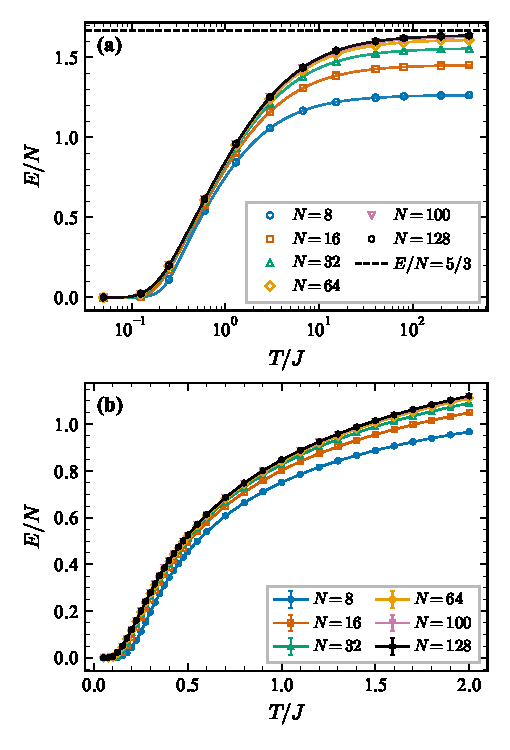
\includegraphics[width=0.48\linewidth]{fig3_energy.pdf}
  \hfill
  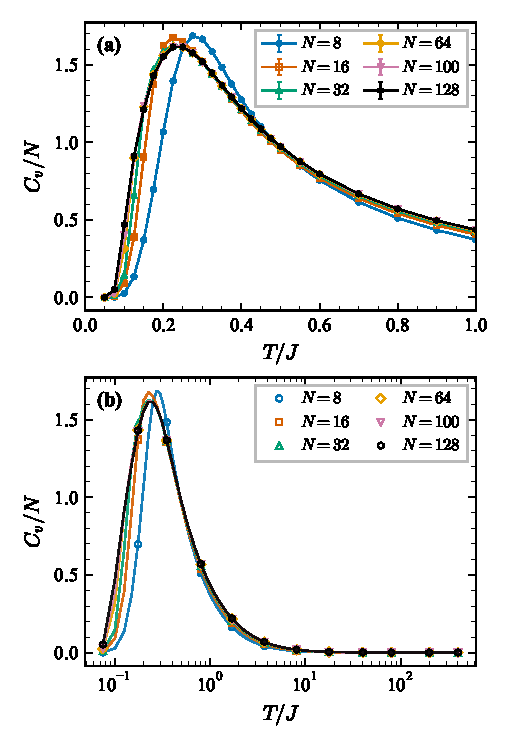
\includegraphics[width=0.48\linewidth]{fig4_cv.pdf}
  \caption{(a)~Energy per queen $E/N$ vs temperature for
  $N = 8$--128.  The dashed line marks the analytical
  $N \to \infty$ limit $E/N = 5/3$.
  (b)~Specific heat per queen $C_v/N$ vs temperature.
  For $N \ge 32$ the curves collapse onto a universal function
  with a non-divergent peak $C_v^{\max}/N \approx 1.62$.}
  \label{fig:thermo}
\end{figure}

\begin{table}[b]
\caption{Specific heat peak scaling.  The peak height saturates
for $N \ge 32$, ruling out a phase transition.}
\centering
\begin{tabular}{l c c c}
\hline
$N$ & $T_{\rm peak}/J$ & $C_v^{\max}/N$ & Error \\
\hline
8   & 0.281 & 1.692 & 0.0002 \\
16  & 0.227 & 1.678 & 0.0006 \\
32  & 0.231 & 1.629 & 0.0005 \\
64  & 0.237 & 1.622 & 0.0004 \\
100 & 0.237 & 1.623 & 0.0004 \\
128 & 0.237 & 1.623 & 0.0004 \\
\hline
\end{tabular}
\label{tab:cv_peak}
\end{table}

\textit{Thermodynamic integration.}---The convergence of $C_v/N$ to
a universal function enables a powerful self-consistency check.  At
$T \to \infty$, the entropy per queen is exact:
\begin{equation}
  \frac{S(\infty)}{N}
  = \frac{1}{N}\ln\binom{N^2}{N}
  = \ln N + 1 + O\!\left(\frac{\ln N}{N}\right).
  \label{eq:Sinf}
\end{equation}
At $T = 0$, only ground states contribute:
$S(0)/N = \ln Q(N)/N \approx \ln N - \gamma$.
The fundamental thermodynamic relation
\begin{equation}
  \frac{S(\infty) - S(0)}{N}
  = \int_0^\infty \frac{C_v}{NT}\,dT
  = 1 + \gamma + O\!\left(\frac{\ln N}{N}\right)
  \label{eq:DS}
\end{equation}
connects the MC specific heat data to the combinatorial constant
$\gamma$.  Rearranging, the ground-state entropy is extracted as
\begin{equation}
  s_0^{\rm MC}
  = \frac{S(\infty)}{N} - \int_0^\infty \frac{C_v}{NT}\,dT,
  \label{eq:s0_MC}
\end{equation}
providing a purely thermodynamic determination of the ground-state
degeneracy without direct enumeration.

Table~\ref{tab:entropy} summarizes the results.  For $N = 8$ and
16, where exact values of $Q(N)$ are known ($Q(8) = 92$,
$Q(16) = 14\,772\,512$), $s_0^{\rm MC}$ agrees with
$s_0^{\rm exact} = \ln Q(N)/N$ to within 1.2\% and 0.5\%
respectively, validating the procedure.  For $N \ge 32$, the
extracted Simkin constant
$\gamma_{\rm MC} = \ln N - s_0^{\rm MC}$ converges toward the
combinatorial value: $\gamma_{\rm MC} = 1.83$ ($N = 32$),
$1.89$ ($N = 64$), $1.92$ ($N = 128$), and $1.94$ ($N = 512$),
with the deviation decreasing from $5.9\%$ to $0.07\%$.
The dominant source of error at moderate $N$ is the finite-size
correction to the Simkin formula, which makes
$\gamma_{\rm eff}(N) = \ln N - s_0(N)$ systematically smaller
than the asymptotic $\gamma$; the MC integration itself introduces
only sub-percent errors, as confirmed by the $N = 8$ and 16
benchmarks.

\begin{table}[t]
\caption{Ground-state entropy from thermodynamic integration.
For $N \le 16$, $s_0^{\rm MC}$ is compared with the exact value.
For $N \ge 32$, $\gamma_{\rm MC} = \ln N - s_0^{\rm MC}$ is
compared with $\gamma \in [1.939,\, 1.945]$~[2].}
\centering
\begin{tabular}{l c c c c}
\hline
$N$ & $s_0^{\rm MC}$ & $s_0^{\rm exact}$ & $\gamma_{\rm MC}$
    & Deviation \\
\hline
8   & 0.558 & 0.565 & ---   & 1.2\% \\
16  & 1.027 & 1.032 & ---   & 0.5\% \\
\hline
32  & 1.639 & ---   & 1.827 & 5.9\% \\
64  & 2.268 & ---   & 1.891 & 2.6\% \\
100 & 2.704 & ---   & 1.901 & 2.1\% \\
128 & 2.931 & ---   & 1.922 & 1.0\% \\
256 & 3.625 & ---   & 1.920 & 1.1\% \\
512 & 4.298 & ---   & 1.941 & 0.07\% \\
\hline
\end{tabular}
\label{tab:entropy}
\end{table}

\textit{Discussion.}---We have presented a statistical-mechanical
investigation of the $N$-queens lattice gas through extensive MC
simulations.  Our main findings are: (i)~the ground-state entropy
$s_0 = \ln N - \gamma$ decomposes through a constraint hierarchy
in which the column constraint costs exactly 1 unit while the two
diagonal constraints cost $\gamma - 1 \approx 0.94$ units;
(ii)~the exact high-temperature energy $E/N \to 5/3$;
(iii)~the specific heat $C_v/N$ converges to a universal function
whose non-divergent peak rules out a phase transition;
(iv)~thermodynamic integration recovers $\gamma$ to within $0.1\%$
at $N = 512$, providing the first physical determination of this
combinatorial constant.

The remarkable relation~(\ref{eq:DS}) bridges combinatorics and
thermodynamics: the left side involves MC data across all
temperatures, while the right side involves only the Stirling
correction (the constant 1) and the Simkin constant $\gamma$.
This demonstrates that a single MC campaign can determine a
fundamental combinatorial constant through the laws of
thermodynamics.

A natural extension is to simulate larger systems ($N \gtrsim 512$)
for more precise thermodynamic determination of $\gamma$, and to
apply this approach to other constraint satisfaction problems where
exact enumeration is unavailable.

\section*{References}

\begin{enumerate}
\renewcommand{\labelenumi}{[\theenumi]}

\item Bezzel M 1848 \textit{Berliner Schachzeitung} \textbf{3} 636

\item Simkin M 2023 \textit{Adv.\ Math.} \textbf{427} 109127

\item Bowtell C and Keevash P 2021 The $n$-queens problem
  (arXiv:2109.08083)

\item Luria Z and Simkin M 2021 A lower bound for the $n$-queens
  problem (arXiv:2105.11431)

\item Knuth D E 2022 \textit{The Art of Computer Programming}
  vol~4B (Boston: Addison-Wesley) sec~7.2.2

\item Kawasaki K 1966 \textit{Phys.\ Rev.} \textbf{145} 224

\item Metropolis N, Rosenbluth A W, Rosenbluth M N, Teller A H
  and Teller E 1953 \textit{J.\ Chem.\ Phys.} \textbf{21} 1087

\item Binder K and Heermann D W 2010 \textit{Monte Carlo
  Simulation in Statistical Physics} 5th edn (Berlin: Springer)

\item Zhang C and Ma J 2009 \textit{Phys.\ Rev.\ E} \textbf{79}
  016703

\item Polson N and Sokolov V 2024 Counting $N$ queens
  (arXiv:2407.08830)

\end{enumerate}

\end{document}
